\documentclass{article}

\usepackage[english]{babel}
\usepackage[utf8]{inputenc}
\usepackage{amsmath,amssymb}
\usepackage{parskip}
\usepackage{graphicx}
\usepackage{rotating}
\usepackage[top=2.5cm, left=3cm, right=3cm, bottom=4.0cm]{geometry}
\usepackage[toc,page]{appendix}

\usepackage[table]{xcolor}


\newcommand{\tablespace}{\\[1.25mm]}
\newcommand\Tstrut{\rule{0pt}{2.6ex}}
\newcommand\tstrut{\rule{0pt}{2.0ex}}
\newcommand\Bstrut{\rule[-0.9ex]{0pt}{0pt}}

\title{CO395 - Machine Learning Coursework 1}
\author{
    Padmanaba Srinivasan \\
    \texttt{01191525}
    \and
    Keerthanen Ravichandran \\
    \texttt{01195170}
    \and
    Harrison Ankers \\
    \texttt{01211208}
    \and
    Tze Hei Tang \\
    \texttt{01221240}
}
\date{\today}

\begin{document}
\maketitle
\newpage
\tableofcontents
\newpage

\section{Construction of the Decision Tree}
\subsection{Brief overview of building the decision tree}
The following describes algorithm that builds the decision tree given a dataset.
\begin{enumerate}
    \item Begin by creating a root node, then split the dataset at the point which provides the maximum information gain.
    \item Recursively build subtrees using the subsets, which form left and right branches on the root node.
    \item When no further splitting is possible, form leaf nodes which contain room values.
\end{enumerate}

\subsection{How we selected the best attribute in each node}
The attribute with the maximum information gain is used as the splitting point to form subsets.\\
The information gain is calculated as follows:\\
\begin{align}
    \label{decisiontree:f1}
	 G(q) = H(dataset) - (  \frac{|subsetA|}{|dataset|} H(subsetA) + \frac{|subsetB|}{dataset} H(subsetB) )
    \end{align}
Where H(p) is the entropy of the data set p, denoted by:
\begin{align}
    \label{decisiontree:f2}
    H(dataset) = - \sum_{k}^{N} d_{k}log_{2}(d_{k})
\end{align}
where $d_{k}$ denotes the $k^{th}$ element in data set D with N elements\\

Hence, from the above expressions, a threshold value that separates the original data set into data set A and B is selected such that the gain expression is maximised.

In order to achieve the above, we iterate through a sorted version of the data set that corresponds to the current node, and we try to separate the data set into A and B by setting the threshold to $\frac{d_{i} + d_{i+1}}{2}$.

Now, the entropy of data set A and B, and the corresponding information gain are computed according to equations $(\ref{decisiontree:f1})$ and $(\ref{decisiontree:f2})$. The threshold that gives the highest information gain is selected, and the data set is split into subsets A and B, where: $$A_{i} < threshold $$ $$B_{j} \geq threshold$$
\\
The dataset A now corresponds to the left child node, and data set B to the right child node. This process is repeated recursively.
\\\\
Eventually, a leaf has to be created at the end of a branch; there are three conditions in which a leaf is created.
\begin{enumerate}
    \item When either A or B is an empty set, the modal room value original data set is used as the final value of the leaf.
    \item When the all of the attribute values in the original dataset is the same, the modal room number is used as the value of the leaf.
    \item When all of the room values in a dataset are the same, further splitting cannot occur so a leaf node is created with the room number.
\end{enumerate}

%%%%%%%%%%%%%%%%%%%%%%%%%%%%%%%%%%%%%%%%%%%%%%%%%%%%%%%%%%%%%%%%%%%%%%%%%%%
%									Cross - Validation
%%%%%%%%%%%%%%%%%%%%%%%%%%%%%%%%%%%%%%%%%%%%%%%%%%%%%%%%%%%%%%%%%%%%%%%%%%%
\section{10 Fold Cross Validation}

\subsection{Why Cross Validation?}
Cross Validation is a technique employed to produce and evaluate the best possible model when the number of samples is low. The dataset is separated into $k$ folds with one fold used as a test set, another as a validation set and the remaining $k-2$ as training data. Repeating this with all possible combinations of training and validation sets will produce $k(k-1)$ tests overall. Evaluation of each model can be performed on the confusion matrix it yields when tested.

In this project, $k=10$ and 90 trees are trained.

\subsection{Cross Validation Implementation}

Given the entire dataset and $k$=10, the size of each fold can be calculated. Following this the dataset is shuffled once and then a fold removed to form the test set. Of the remaining $k-1$ folds, another fold forms the validation set with the residual data making up the training data. This is implemented by having two loops, with the outer loops separating out the test set and the inner loop generating the training and validation set. As a result, every fold gets the opportunity to be test set validation set once each.

After a tree is trained on the training data, its' error rate on test set is found and the confusion matrix analysed (to calculate recall and precision rates as well as F1 values) before the tree is pruned and the new confusion matrix analysed again. Having two sets of confusion matrices both before and after pruning is a useful tool in comparing the effectiveness of pruning.

This procedure is repeated to train 90 trees and test and evaluate 180 trees overall.



\section{Questions}

\subsection{Pruning}

\subsubsection{Pruning Implementation}

Pruning is implemented via the $Pruning$ class in $lib$ which is initialised with a validation set and once built, the root of the tree is passed in for automatic Pruning.

Pruning involves firstly testing the validation set on the tree and obtaining an error rate. Following this the $prunify$ function is called which recursively finds nodes which is the parent of two leaves directly. At this stage there are two possible paths: firstly to make the node a leaf or secondly to keep the decision node as is. The obtains the leaf values from both child nodes and calculates the error rate if the decision node were a leaf with each value. If error rate improves then the best improvement is chosen, the decision node converted into a leaf with this value and the best error rate updated. If pruning does not provide an improvement then the decision node is kept as is.

Another method of pruning is to use Error-Estimation (EE) \cite{eeprune}, commonly used with the C4.5 algorithm. This method takes a more statistical approach and is similar in structure to the standard algorithm. With EE the dataset itself \'travels\' down the tree, splitting on each decision node. When a set reaches a leaf, the leaf calculates the actual error rate a well as the estimated error rate with the formula in figure \ref{pruning:f1}. Both these error rates are returned. Following this the decision node calculates the weighted sum of the error rate of its' leaves to find the node error, and the weighted sum of the estimated error to find the subtree error. Pruning occurs if the node error is larger than the subtree error. This repeats recursively \'up\' the tree. An illustration of this is in figure \ref{pruning:d1}. EE is implemented within the Node class and is called upon as a member function, passing in the validation set as a parameter.


\begin{align}
\label{pruning:f1}
	 e = \frac{ f + \frac{z^2}{2N} + z\sqrt{\frac{f}{N} + \frac{f^2}{N} + \frac{z^2}{4N^2}}  } {1 + \frac{z^2}{N}}
\end{align}

\begin{figure}
\centering
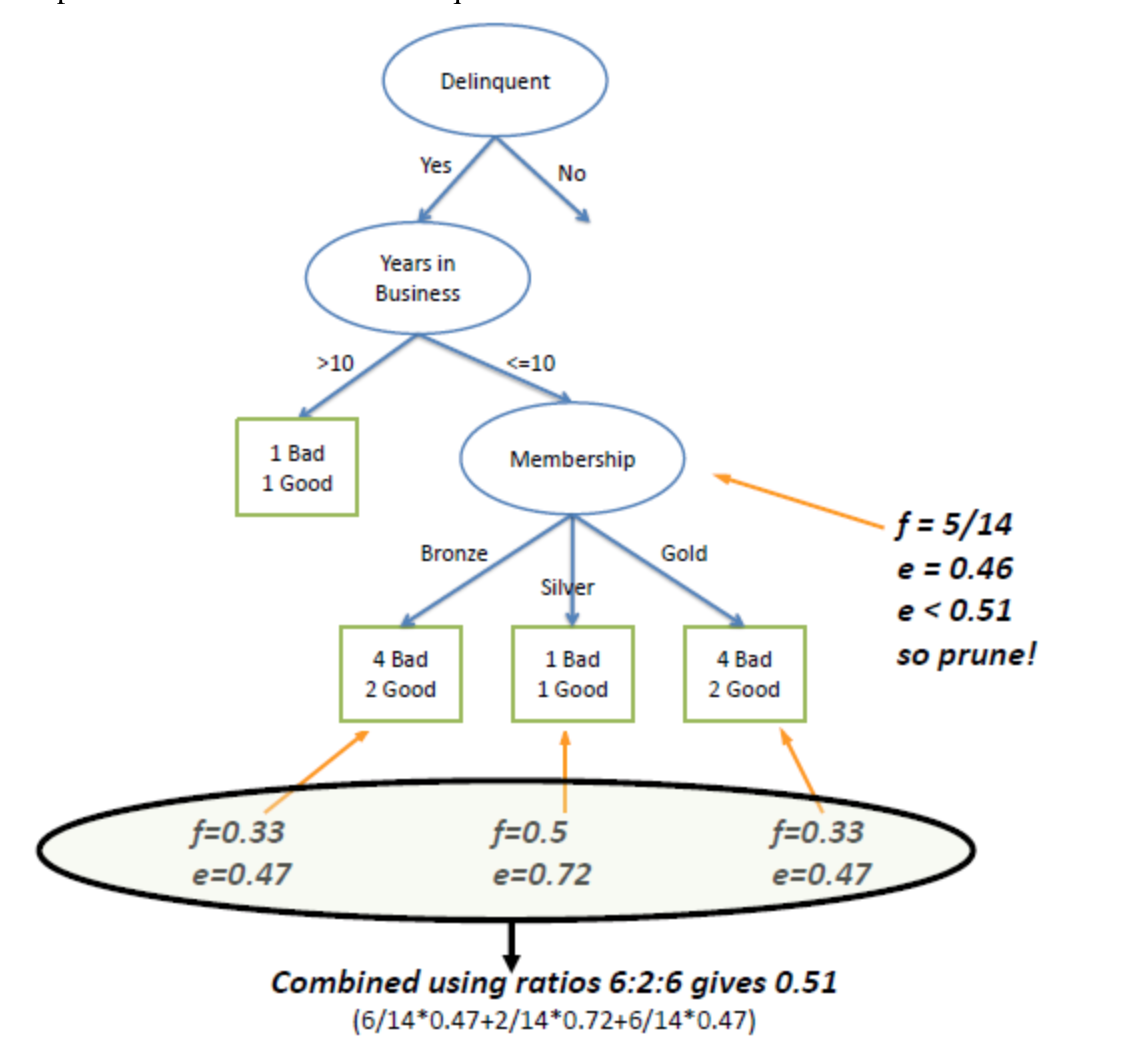
\includegraphics[width=0.7\textwidth]{figures/pruningd1.png}
\caption{\label{pruning:d1} An illustration of pruning with Error-Estimation. }
\end{figure}

Testing both methods of pruning with the noisy dataset showed clear advantages to EE; from a high level the standard method for pruning improved noisy dataset classification rate by around 1\% overall, whereas pruning using EE has a more significant effect, typically improving classification rate by 2-5\%.

Looking at the number of nodes after pruning with each method yields some insights. Figure \ref{pruning:s1} shows number of nodes before and after pruning with each method. The trees provided to both prune algorithms were trained on the same training set and so were identical.


\begin{figure}
\centering
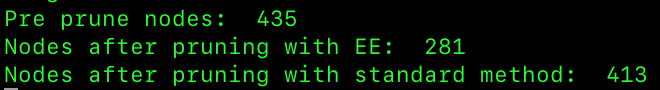
\includegraphics[width=0.7\textwidth]{figures/prunings1.png}
\caption{\label{pruning:s1} Comparing the number of nodes with different pruning methods. }
\end{figure}

\begin{figure}
\centering
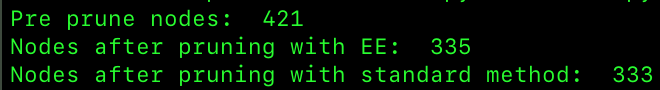
\includegraphics[width=0.7\textwidth]{figures/prunings2.png}
\caption{\label{pruning:s2} Pruning with EE followed by the standard method. }
\end{figure}

\begin{figure}
\centering
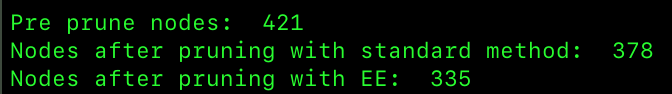
\includegraphics[width=0.7\textwidth]{figures/prunings3.png}
\caption{\label{pruning:s3} Pruning with the standard method followed by EE. }
\end{figure}



Combining these methods, pruning with EE first followed by the standard method yields metrics in figure \ref{pruning:s2} and then reversing the order, pruning vice-verse yields figure \ref{pruning:s3}. In both cases, the datasets (all derived from the noisy dataset) used were the same and so the initial decision tree to was the same. In this example using the standard pruning method after the aggressive EE pruning yields a slightly smaller tree. Over several different datasets, the second method yielded trees of the same size or slightly larger than trees produced by the first method. Correspondingly, the classification rates were the same or slightly larger for the first method overall.

Using combined pruning algorithms yielded slightly higher classification rates than using any one algorithm on its own and showed a clear inverse link between tree size and classification rate. With any pruning algorithm, trees derived from the clean dataset little change in the number of nodes or classification rate.

\subsubsection{Pruning's effects on Classification Rate}

Observing the classification rate for a number of folds on the clean dataset reveals little change in classification rate, with classification rate typically changing by less than 0.5\% post pruning. Decreases in the classification rate are more common and can be expected as the purpose of pruning is to reduce overfitting. The clean dataset is so because it doesn't overfit much to begin with and whatever pruning occurs changes classification rate minimally, with classification rate hovering around 97\% before and after pruning. This seems feasible given the observation that the size of the tree remains the same after pruning despite the methods.

The noisy dataset however, tells a very different story. Pre-pruning, the tree's accuracy hovers around 80-81\%. Pruning with the standard method only improves classification rate from 1-2\% boosting it up to 81-82\%. Using only EE typically boosts classification rate to around 84\% and combining methods yields the same improvement. The small difference in using only EE and combining methods is explained by EE aggressively pruning most of the tree leaving the standard method to prune very little.

Overall, pruning has little effect on classification rate in the clean dataset which is evidenced by little to no reduction in the number of nodes in the tree, with there being around 60 nodes on average and pruning reducing this by around 20\%. In some, rare, extreme cases the number of nodes decreased by 50\%, although classification rate remained constant.

With the noisy dataset the number of nodes drops from around 400-450 to around 300-330, roughly a 25\% reduction in tree size overall. This suggests rampant overfitting on the noisy dataset which is alleviated by pruning but even still is in stark contrast to training on clean data. Also, noticing the difference in sheer number of nodes in trees between the clean and noisy datasets despite training data being of same size, there seems to be a link between the noisiness of the data and the degree to which it is overfitted. This logically leads onto the question of whether data can be cleaned before it is used and whether an indicator of noisy data could be related to the size of the decision tree it produces.

\subsection{Metrics in Clean and Noisy Datasets}

\subsubsection{Metrics}

Various metrics can be obtained from the tests to assess the performance of the tree. Specifically performance can also be analysed by looking at metrics such as classification rate, recall, and F1 measure.

\subsubsection{Performance}

The classification rate displays the percentage of correctly identified elements as a proportion of the whole test set. The pre prune, clean and noisy datasets produced the confusion matrices in tables \ref{clean_preprune} and \ref{noisy_preprune} respectively. The metrics derived from these matrices are in table \ref{avg_metrics}.

Recall rate indicates how many of the actual positive results are classified as positive by the model which for the clean data is very high. Similarly, precision rate - which is a measure of the correct positive predictions as a proportion of total positive predictions - too is high. Correspondingly, the F1 rate too is high. These indicate a high level confidence that the model will correctly classify inputs. The fact the F1 is so close to 1 for both pre prune and post prune indicates that this tree is close of perfect precision and recall.

Post pruning, for the model trained on clean data the recall and precision rates change very little indicating that this method of pruning cannot improve prediction accuracy much further.

The metrics for the noisy dataset however, tell a different story. Both precision rate and recall rate are lower indicating a more spread out confusion matrix where fewer positive predictions and correct and fewer positive values are classified as being positive. Post pruning the metrics increase by around 4.5\% all round, with the increase in F1 showing that the model is getting closer to perfect precision and recall.

\subsubsection{Pruning performance}

Pruning optimises the tree via pruning off leaves that cause overfitting on a validation set, following which the pruned model is tested on the test data once more. It is expected that model performs better on the test data after pruning.

When tested with clean data the classification rate was 97.1\%. Furthermore, when tested with noisy data the rate again lowered to 84.85\%. The clean data classification matrix only slightly increased, though, the noisy data had a larger increase. Both clean and noisy data produced the confusion matrices in tables \ref{clean_preprune} and \ref{noisy_preprune} respectively. Post prune tables are in tables \ref{clean_postprune} and \ref{noisy_postprune}. The clean data produced an average recall of 97.12\% and the noisy produced a recall of 84.86\%. The clean data showed almost no improvement, however, the noisy data had a more dramatic increase. The clean data produced an average F1 of 97.11\% and the noisy produced a F1 of 84.86\%. The F1 metric showed a slight decrease in performance for the clean data, however, the noisy data improved again.

On the clean dataset, pre pruning classification rate was 97.2\% and fell slightly to 97.1\% post pruning. This can be attributed to the data being pruned on the validation set, which by extension reduces overfitting on the test data and attempts to fit the model more to the validation set. Over several repetitions there was no consistent trend in post prune classification rate, sometimes being lower and sometimes higher.

The noisy dataset however, yields some important insights into the effectiveness of pruning. Pre prune classification rate stood at 80.3\% which increased to 84.85\% post prune. This is a significant improvement and again over several repetitions pruning improved classification rate by 3-4\%.



\begin{table}[]
\begin{tabular}{|c|c|c|c|c|}
\hline
 & \textbf{\begin{tabular}[c]{@{}c@{}}Room 1 \\ (Actual)\end{tabular}} & \textbf{\begin{tabular}[c]{@{}c@{}}Room 2 \\ (Actual)\end{tabular}} & \textbf{\begin{tabular}[c]{@{}c@{}}Room 3 \\ (Actual)\end{tabular}} & \textbf{\begin{tabular}[c]{@{}c@{}}Room 4 \\ (Actual)\end{tabular}} \\ \hline
\textbf{\begin{tabular}[c]{@{}c@{}}Room 1 \\ (Predicted)\end{tabular}} & 49.4 & 0 & 0.2 & 0.5 \\ \hline
\textbf{\begin{tabular}[c]{@{}c@{}}Room 2 \\ (Predicted)\end{tabular}} & 0 & 47.6 & 1.6 & 0 \\ \hline
\textbf{\begin{tabular}[c]{@{}c@{}}Room 3 \\ (Predicted)\end{tabular}} & 0.4 & 2.4 & 48.1 & 0.2 \\ \hline
\textbf{\begin{tabular}[c]{@{}c@{}}Room 4 \\ (Predicted)\end{tabular}} & 0.2 & 0 & 0.1 & 49.3 \\ \hline
\end{tabular}
\caption{Confusion Matrix (clean data pre-prune)}
\label{clean_preprune}
\end{table}

\begin{table}[]
\begin{tabular}{|c|c|c|c|c|}
\hline
 & \textbf{\begin{tabular}[c]{@{}c@{}}Room 1 \\ (Actual)\end{tabular}} & \textbf{\begin{tabular}[c]{@{}c@{}}Room 2 \\ (Actual)\end{tabular}} & \textbf{\begin{tabular}[c]{@{}c@{}}Room 3 \\ (Actual)\end{tabular}} & \textbf{\begin{tabular}[c]{@{}c@{}}Room 4 \\ (Actual)\end{tabular}} \\ \hline
\textbf{\begin{tabular}[c]{@{}c@{}}Room 1 \\ (Predicted)\end{tabular}} & 38.7 & 3.3 & 2.8 & 3.5 \\ \hline
\textbf{\begin{tabular}[c]{@{}c@{}}Room 2 \\ (Predicted)\end{tabular}} & 3.7 & 40 & 3.9 & 2.1 \\ \hline
\textbf{\begin{tabular}[c]{@{}c@{}}Room 3 \\ (Predicted)\end{tabular}} & 3.2 & 3.5 & 41.5 & 3.8 \\ \hline
\textbf{\begin{tabular}[c]{@{}c@{}}Room 4 \\ (Predicted)\end{tabular}} & 3.4 & 2.9 & 3.3 & 40.4 \\ \hline
\end{tabular}
\caption{Confusion Matrix (noisy data pre-prune)}
\label{noisy_preprune}
\end{table}


\begin{table}[]
\begin{tabular}{l|l|l|l|l|}
\cline{2-5}
 & \multicolumn{2}{l|}{Clean Data} & \multicolumn{2}{l|}{Noisy Data} \\ \cline{2-5}
 & Pre-pruning & Post-pruning & Pre-pruning & Post-pruning \\ \hline
\multicolumn{1}{|l|}{Avg. Precision} & 97.20\% & 97.10\% & 80.30\% & 84.85\% \\ \hline
\multicolumn{1}{|l|}{Avg. Recall} & 97.22\% & 97.12\% & 80.30\% & 84.86\% \\ \hline
\multicolumn{1}{|l|}{Avg. F1} & 97.20\% & 97.11\% & 80.30\% & 84.86\% \\ \hline
\end{tabular}
\caption{Metrics from confusion matrices}
\label{avg_metrics}
\end{table}

\begin{table}[]
\begin{tabular}{|c|c|c|c|c|}
\hline
 & \textbf{\begin{tabular}[c]{@{}c@{}}Room 1 \\ (Actual)\end{tabular}} & \textbf{\begin{tabular}[c]{@{}c@{}}Room 2 \\ (Actual)\end{tabular}} & \textbf{\begin{tabular}[c]{@{}c@{}}Room 3 \\ (Actual)\end{tabular}} & \textbf{\begin{tabular}[c]{@{}c@{}}Room 4 \\ (Actual)\end{tabular}} \\ \hline
\textbf{\begin{tabular}[c]{@{}c@{}}Room 1 \\ (Predicted)\end{tabular}} & 49.5 & 0 & 0.2 & 0.5 \\ \hline
\textbf{\begin{tabular}[c]{@{}c@{}}Room 2 \\ (Predicted)\end{tabular}} & 0 & 47.7 & 2 & 0 \\ \hline
\textbf{\begin{tabular}[c]{@{}c@{}}Room 3 \\ (Predicted)\end{tabular}} & 0.5 & 23.0 & 47.7 & 0.2 \\ \hline
\textbf{\begin{tabular}[c]{@{}c@{}}Room 4 \\ (Predicted)\end{tabular}} & 0 & 0 & 0.1 & 49.3 \\ \hline
\end{tabular}
\caption{Confusion Matrix (clean data post-prune)} \label{clean_postprune}
\end{table}





\begin{table}[]
\begin{tabular}{|c|c|c|c|c|}
\hline
 & \textbf{\begin{tabular}[c]{@{}c@{}}Room 1 \\ (Actual)\end{tabular}} & \textbf{\begin{tabular}[c]{@{}c@{}}Room 2 \\ (Actual)\end{tabular}} & \textbf{\begin{tabular}[c]{@{}c@{}}Room 3 \\ (Actual)\end{tabular}} & \textbf{\begin{tabular}[c]{@{}c@{}}Room 4 \\ (Actual)\end{tabular}} \\ \hline
\textbf{\begin{tabular}[c]{@{}c@{}}Room 1 \\ (Predicted)\end{tabular}} & 42.6 & 2.9 & 2.6 & 2.5 \\ \hline
\textbf{\begin{tabular}[c]{@{}c@{}}Room 2 \\ (Predicted)\end{tabular}} & 1.6 & 41.3 & 3.9 & 1.8 \\ \hline
\textbf{\begin{tabular}[c]{@{}c@{}}Room 3 \\ (Predicted)\end{tabular}} & 2.5 & 3.6 & 42.6 & 2.3 \\ \hline
\textbf{\begin{tabular}[c]{@{}c@{}}Room 4 \\ (Predicted)\end{tabular}} & 2.3 & 1.9 & 2.4 & 43.2 \\ \hline
\end{tabular}
\caption{Confusion Matrix (noisy data post-prune)} \label{noisy_postprune}
\end{table}


The confusion matrices also hold other important information. In the clean data pre prune matrix (table \ref{clean_preprune}) notice that Room 2 and Room 3 are much more likely to be confused for the each other and observing their metrics in table \ref{rmetrics_cl_pp} confirm this with both these rooms having slightly lower precision and recall rates. The situation doesn't change much with these two rooms still being confused for one another post pruning in table \ref{rmetrics_cl_pop}. This ambiguity could be solved by using training Random Forests and taking the modal result when testing on a sample.

Comparing the metrics for the noisy dataset both pre prune and post prune (tables \ref{rmetrics_no_pp} and \ref{rmetrics_no_pop} respectively) show a significant increase across all classes, which is confirmed by observing the pre prune and post prune confusion matrices. Rooms 1 and 4 shows the largest gain in the metrics and recall and precision rates for all classes are roughly the same suggesting that all classes are impacted equally by the noisy data.



\begin{table}[]
\begin{tabular}{|c|c|c|c|c|}
\hline
Metrics                  & \textbf{Room 1} & \textbf{Room 2} & \textbf{Room 3} & \textbf{Room 4} \\ \hline
\textbf{Recall rate}    & 0.986           & 0.967           & 0.941           & 0.994          \\ \hline
\textbf{Precision rate} & 0.988           & 0.952           & 0.962           & 0.986           \\ \hline
\textbf{F1 rate}        & 0.987           & 0.960           & 0.952           & 0.990           \\ \hline
\end{tabular}
\caption{Metrics for clean pre-prune}
\label{rmetrics_cl_pp}
\end{table}

\begin{table}[]
\begin{tabular}{|c|c|c|c|c|}
\hline
Metrics                 & \textbf{Room 1} & \textbf{Room 2} & \textbf{Room 3} & \textbf{Room 4} \\ \hline
\textbf{Recall rate}    & 0.986            & 0.960           & 0.941           & 0.998           \\ \hline
\textbf{Precision rate} & 0.99           & 0.954           & 0.954           & 0.986            \\ \hline
\textbf{F1 rate}        & 0.988           & 0.957           & 0.947          & 0.992           \\ \hline
\end{tabular}
\caption{Metrics for clean post-prune}
\label{rmetrics_cl_pop}
\end{table}

\begin{table}[]
\begin{tabular}{|c|c|c|c|c|}
\hline
Metrics                 & \textbf{Room 1} & \textbf{Room 2} & \textbf{Room 3} & \textbf{Room 4} \\ \hline
\textbf{Recall rate}    & 0.801             & 0.805           & 0.798           & 0.808           \\ \hline
\textbf{Precision rate} & 0.790             & 0.805           & 0.805           & 0.811            \\ \hline
\textbf{F1 rate}        & 0.795             & 0.804            & 0.802           & 0.810           \\ \hline
\end{tabular}
\caption{Metrics for noisy pre-prune}
\label{rmetrics_no_pp}
\end{table}

\begin{table}[]
\begin{tabular}{|c|c|c|c|c|}
\hline
Noisy post prune        & \textbf{Room 1} & \textbf{Room 2} & \textbf{Room 3} & \textbf{Room 4} \\ \hline
\textbf{Recall rate}    & 0.842           & 0.850           & 0.835           & 0.867           \\ \hline
\textbf{Precision rate} & 0.870           & 0.831           & 0.827           & 0.867           \\ \hline
\textbf{F1 rate}        & 0.855           & 0.840            & 0.83          & 0.867           \\ \hline
\end{tabular}
\caption{Metrics for noisy post-prune}
\label{rmetrics_no_pop}
\end{table}


\begin{table}[]
\begin{tabular}{|c|c|}
\label{depths}

\textbf{Datasets}                    & \textbf{Depth} \\ \hline
\textbf{Clean (Pre-prune)}  & 8             \\ \hline
\textbf{Clean (Post-prune)} & 8             \\ \hline
\textbf{Noisy (Pre-prune)}  & 16             \\ \hline
\textbf{Noisy (Post-prune)}  & 13             \\ \hline
\end{tabular}
\caption{Average depths for trees trained on both datasets, pre and post prune.}
\end{table}

\subsection{Depth and Prediction Accuracy}

Looking at the metrics for the noisy dataset, both pre and post prune observe that for all classes the recall, precision and F1 measures increase. This immediately signifies an increase in prediction accuracy. Since pruning has removed nodes and reduced the depth of the tree an relationship exists between reduced depth and increasing prediction accuracy.

The clean dataset sheds further light on this; the prediction accuracy decreases slightly between after pruning despite depth staying the same. As a result a relationship could exist between the extent of pruning and improvements in prediction accuracy. In other words prediction accuracy will increase only if further pruning causes a reduction in depth.

Table \ref{depths} shows that the depth of the decision tree increases with noisy data. In the clean dataset pruning has little effect on depth and suggests that a clean dataset can be identified by little change in depth of the tree when pruned.

By contrast, trees trained on noisy data see a circa 20\% reduction in depth. This further bolsters the theory that noisy datasets correlate with the extent of tree depth reduction. Observing the drop in tree depth and the corresponding increase in classification rate, in general shorter trees imply a higher classification rate as pruning reduces overfitting in the tree, thereby generalising the paths within the tree.



\section{Printing the tree}
The $PrettyPrint$ module uses the $forest$ package in LaTeX to plot a decision tree object. The trees are printed via a recursive function which is then compiled to a pdf.
\\
Figures \ref{cleant:s2} and \ref{noisyt:s2} are the trees trained on the clean and noisy datasets.
\\
Drawings of both trees have also been included as separate pdf's for clarity.

\begin{figure}
\centering
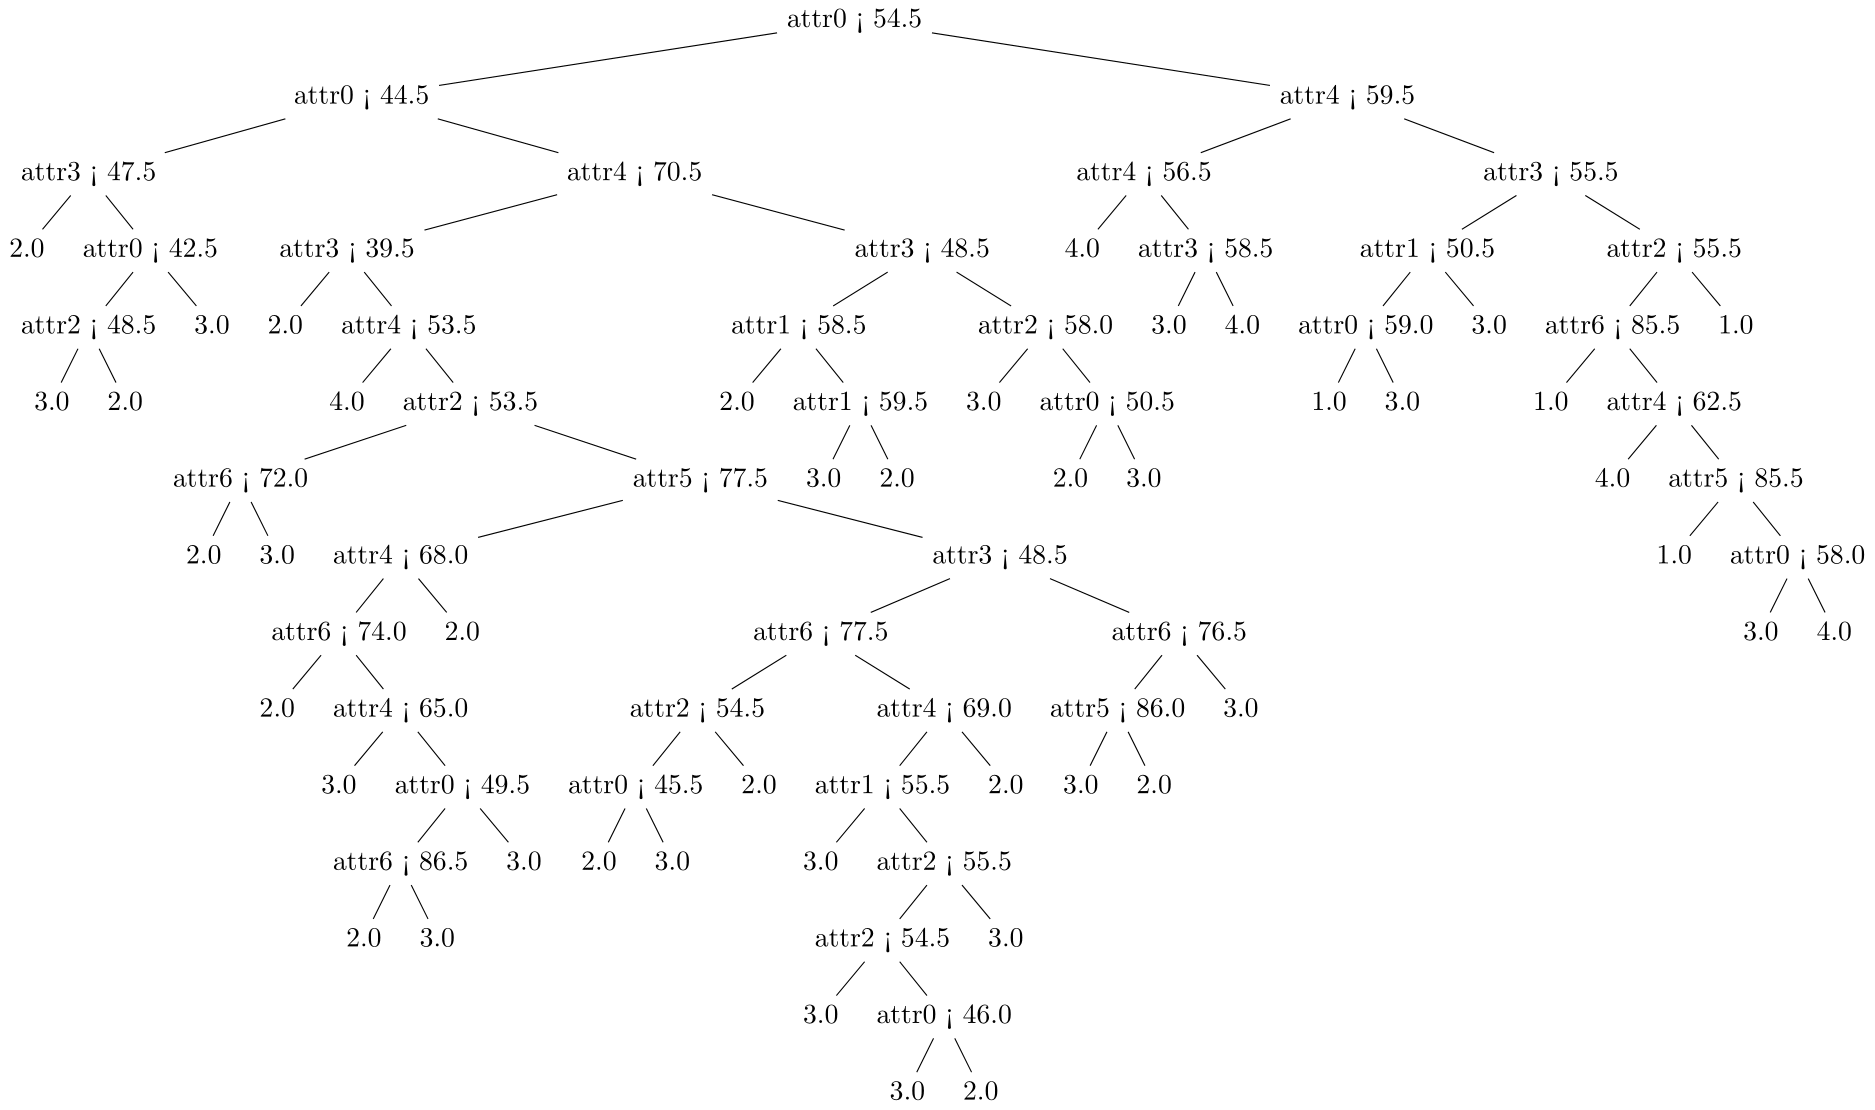
\includegraphics[width=\textwidth,height=\textheight,keepaspectratio]{figures/clean_tree.png}
\caption{ Clean decision tree. }
\label{cleant:s2}
\end{figure}

\vspace{\floatsep}

\newpage

\begin{sidewaysfigure}
\centering

\includegraphics [width=\textwidth,height=\textheight,keepaspectratio]{figures/noisy_tree.png}
\caption{ Noisy decision tree. }
\label{noisyt:s2}
\end{sidewaysfigure}
\clearpage


\section{Bibliography}

\begin{thebibliography}{9}
\bibitem{eeprune}
Dr Saed Sayad, Overfitting. Accessed 25/01/2019
\\\texttt{http://www.saedsayad.com/decision{\_tree\_overfitting.htm}}
\end{thebibliography}

\end{document}
